\section{Auswertung}
\label{sec:Auswertung}
Die Fehlerrechnung wurde mit Unterstützung von Uncertainties \cite{uncertainties} durchgeführt.
\subsection{Statische Methode}
\begin{figure}
	\centering
	\caption{Die Temperatur, am fernem Thermoelement des breiten Messingstabes, $T1$ und, am fernem Thermoelement des schmalen Messingstabes $T4$ gegen die vergangene Zeit $t$ aufgetragen.}
	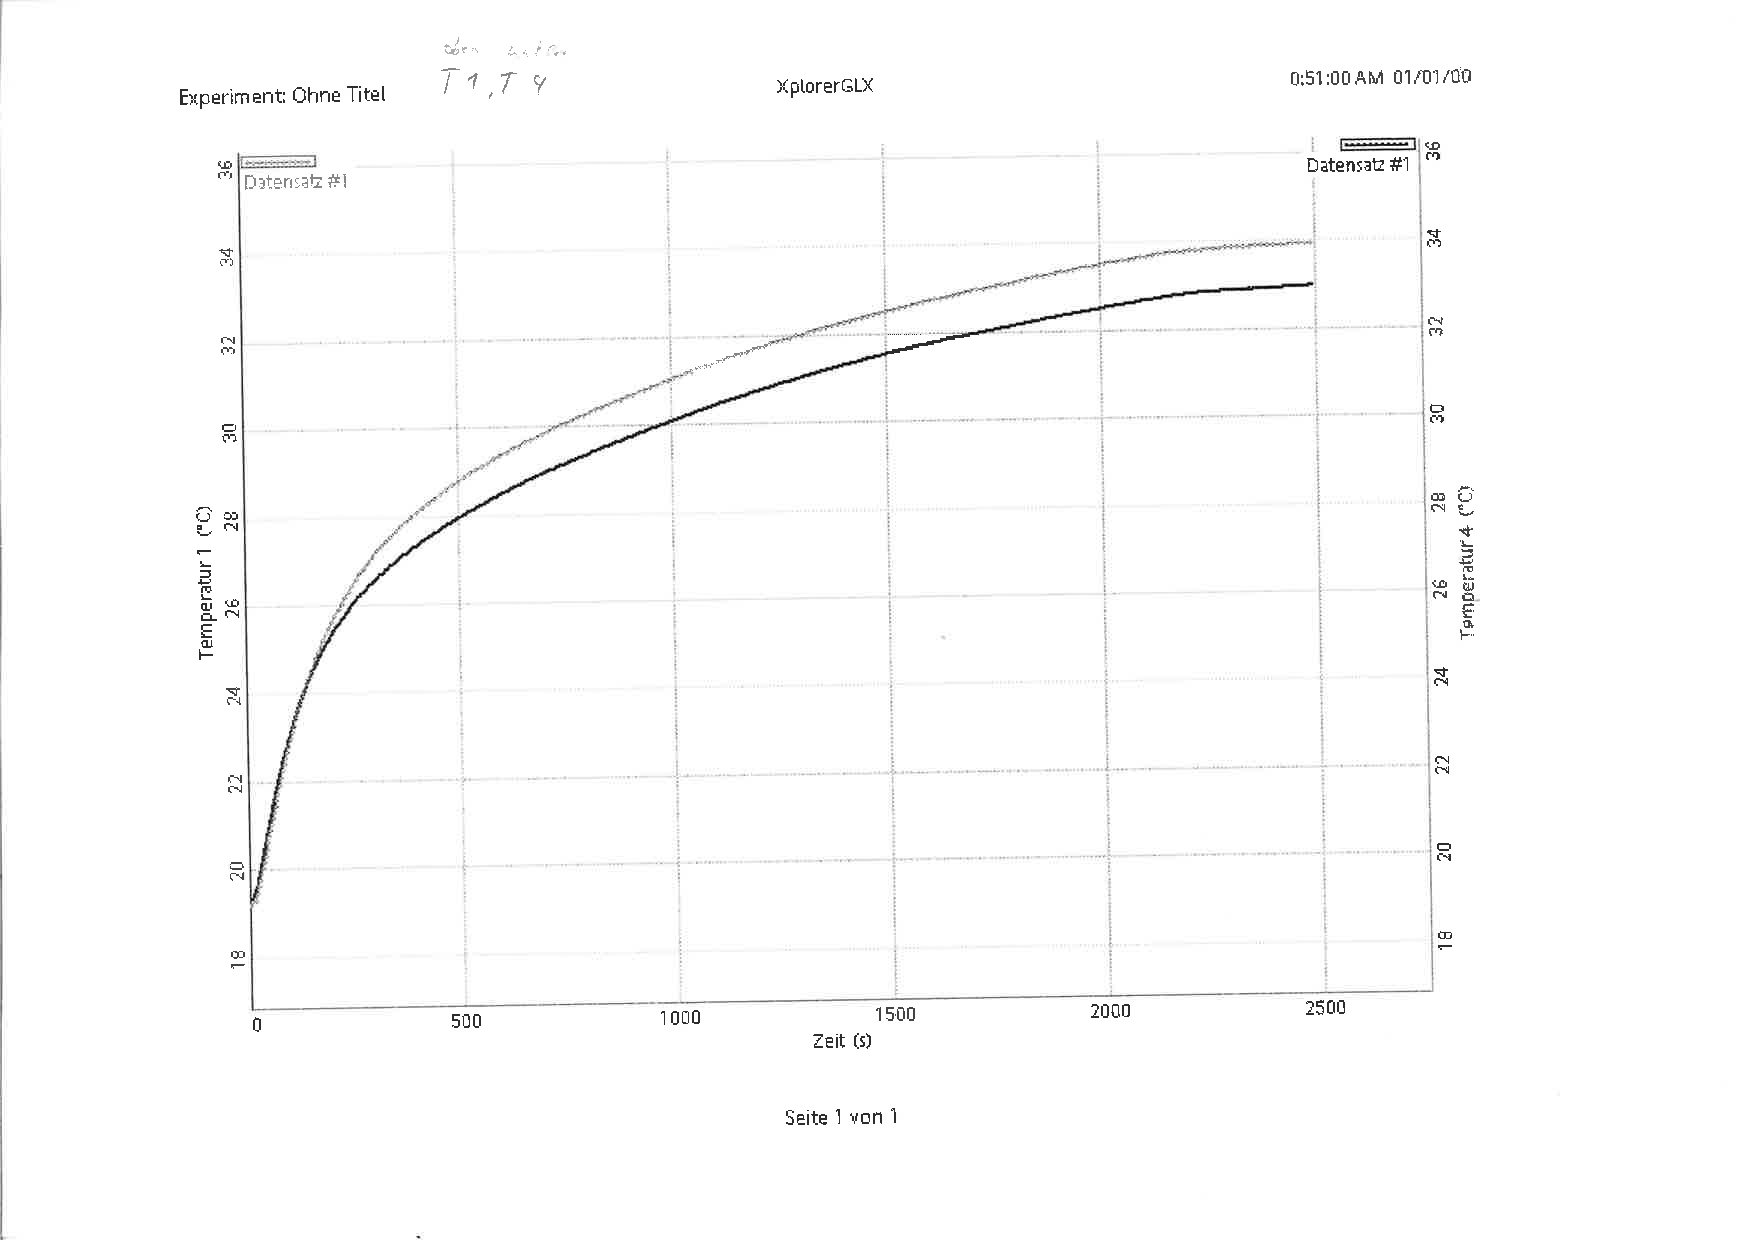
\includegraphics[width=\linewidth-70pt,height=\textheight-70pt,keepaspectratio]{content/Bilder/T1T4-rotated.pdf}
	\label{fig:Graph1}
\end{figure}
In Abbildung \ref{fig:Graph1} sind die Temperaturverläufe an den fernen Thermoelementen der beiden Messingstäbe dargestellt. Es fällt auf, dass in den ersten $\SI{150}{\second}$ beide Temperaturen gleich schnell steigen, danach jedoch die Temperatur am Thermoelement des breitem Stabes $T1$ nicht so früh abflacht, wie $T4$ am schmalem Stab. Die Steigungen der Temperaturverläufe nähern sich im weiterem Verlauf wieder an.
\begin{figure}
	\centering
	\caption{Die Temperatur, am fernem Thermoelement des Aluminiumstabes, $T5$ und, am fernem Thermoelement des Edelstahlstabes, $T8$ gegen die vergangene Zeit $t$ aufgetragen.}
	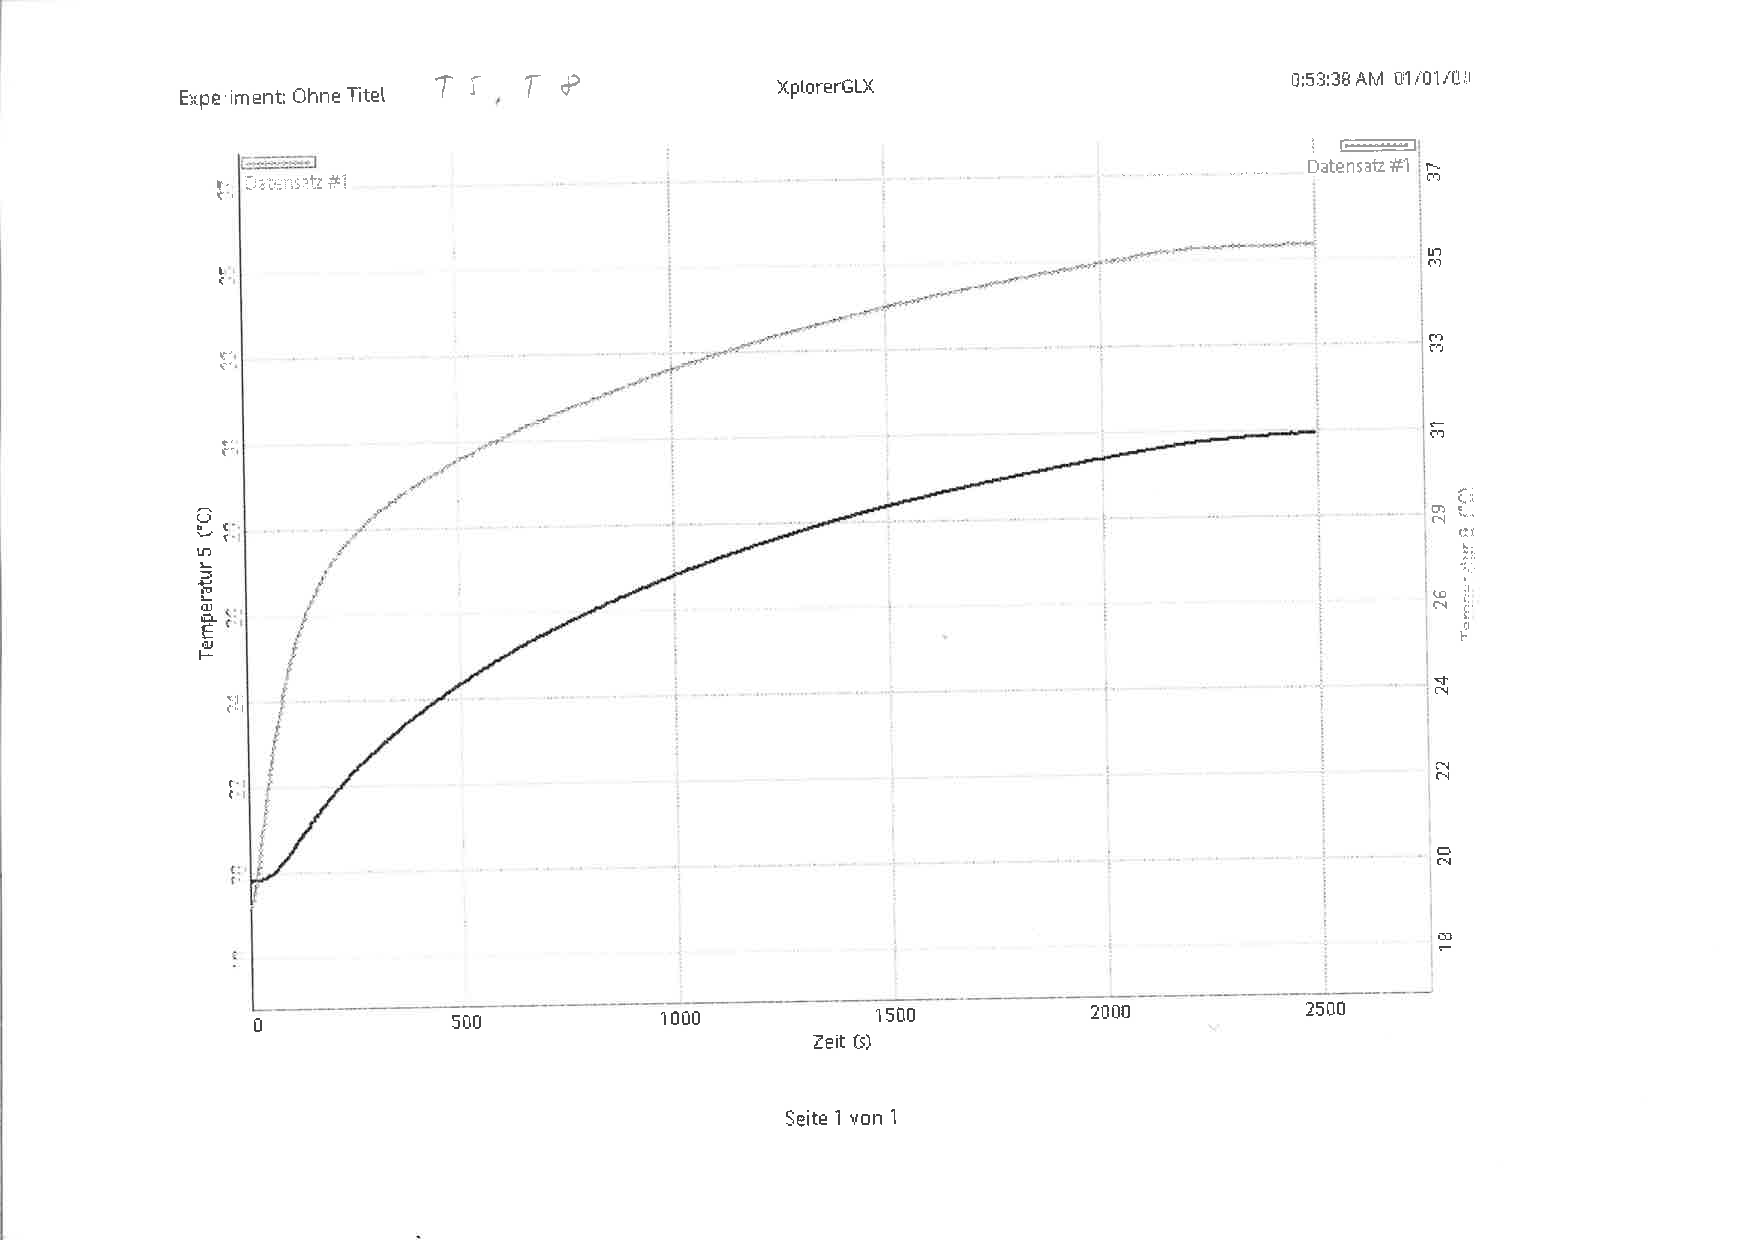
\includegraphics[width=\linewidth-70pt,height=\textheight-70pt,keepaspectratio]{content/Bilder/T5T8-rotated.pdf}
	\label{fig:Graph2}
\end{figure}
In Abbildung \ref{fig:Graph2} ist auch ein Unterschied in den Temperaturverläufen zu erkennen. So beginnt die Temperatur am Edelstahlstab erst später zu steigen als am Aluminiumstab und auch zu Beginn mit einer geringeren Steigung, die sich später der Steigung des Temperaturanstieges am Aluminiumstab annähert.
In allen Graphen in den Abbildungen \ref{fig:Graph1} und \ref{fig:Graph2}  ist direkt bzw. kurz nach Beginn der Messung der größte Temperaturanstieg erkennbar. Dieser fällt bei den unterschiedlichen Materialien unterschiedlich stark aus. Danach nimmt der Anstieg der Temperatur bei allen Graphen ab, wobei sich die Steigungen aneinander annähern. Somit laufen die Graphen gegen unterschiedliche Grenztemperaturen. Die höchste Grenztemperatur besitzt Aluminium, dann Messing und die niedrigste Edelstahl. Dies geht auch schon durch die Temperaturen nach $\SI{700}{\second}$ hervor:
\begin{displaymath}
\begin{aligned}
T5 =& \SI{29.59}{\degreeCelsius}\\
T1 =& \SI{28.09}{\degreeCelsius}\\
T4 =& \SI{27.32}{\degreeCelsius}\\
T8 =& \SI{24.02}{\degreeCelsius}\text{.}
\end{aligned}
\end{displaymath}
Aufgrund der selben Startbedingungen besitzt somit der Aluminiumstab die größte Wärmeleitung.

\begin{figure}
	\centering
	\caption{Die Temperaturdifferenz $T2-T1$ bei dem breitem Messingstab gegen die vergangene Zeit $t$ aufgetragen.}
	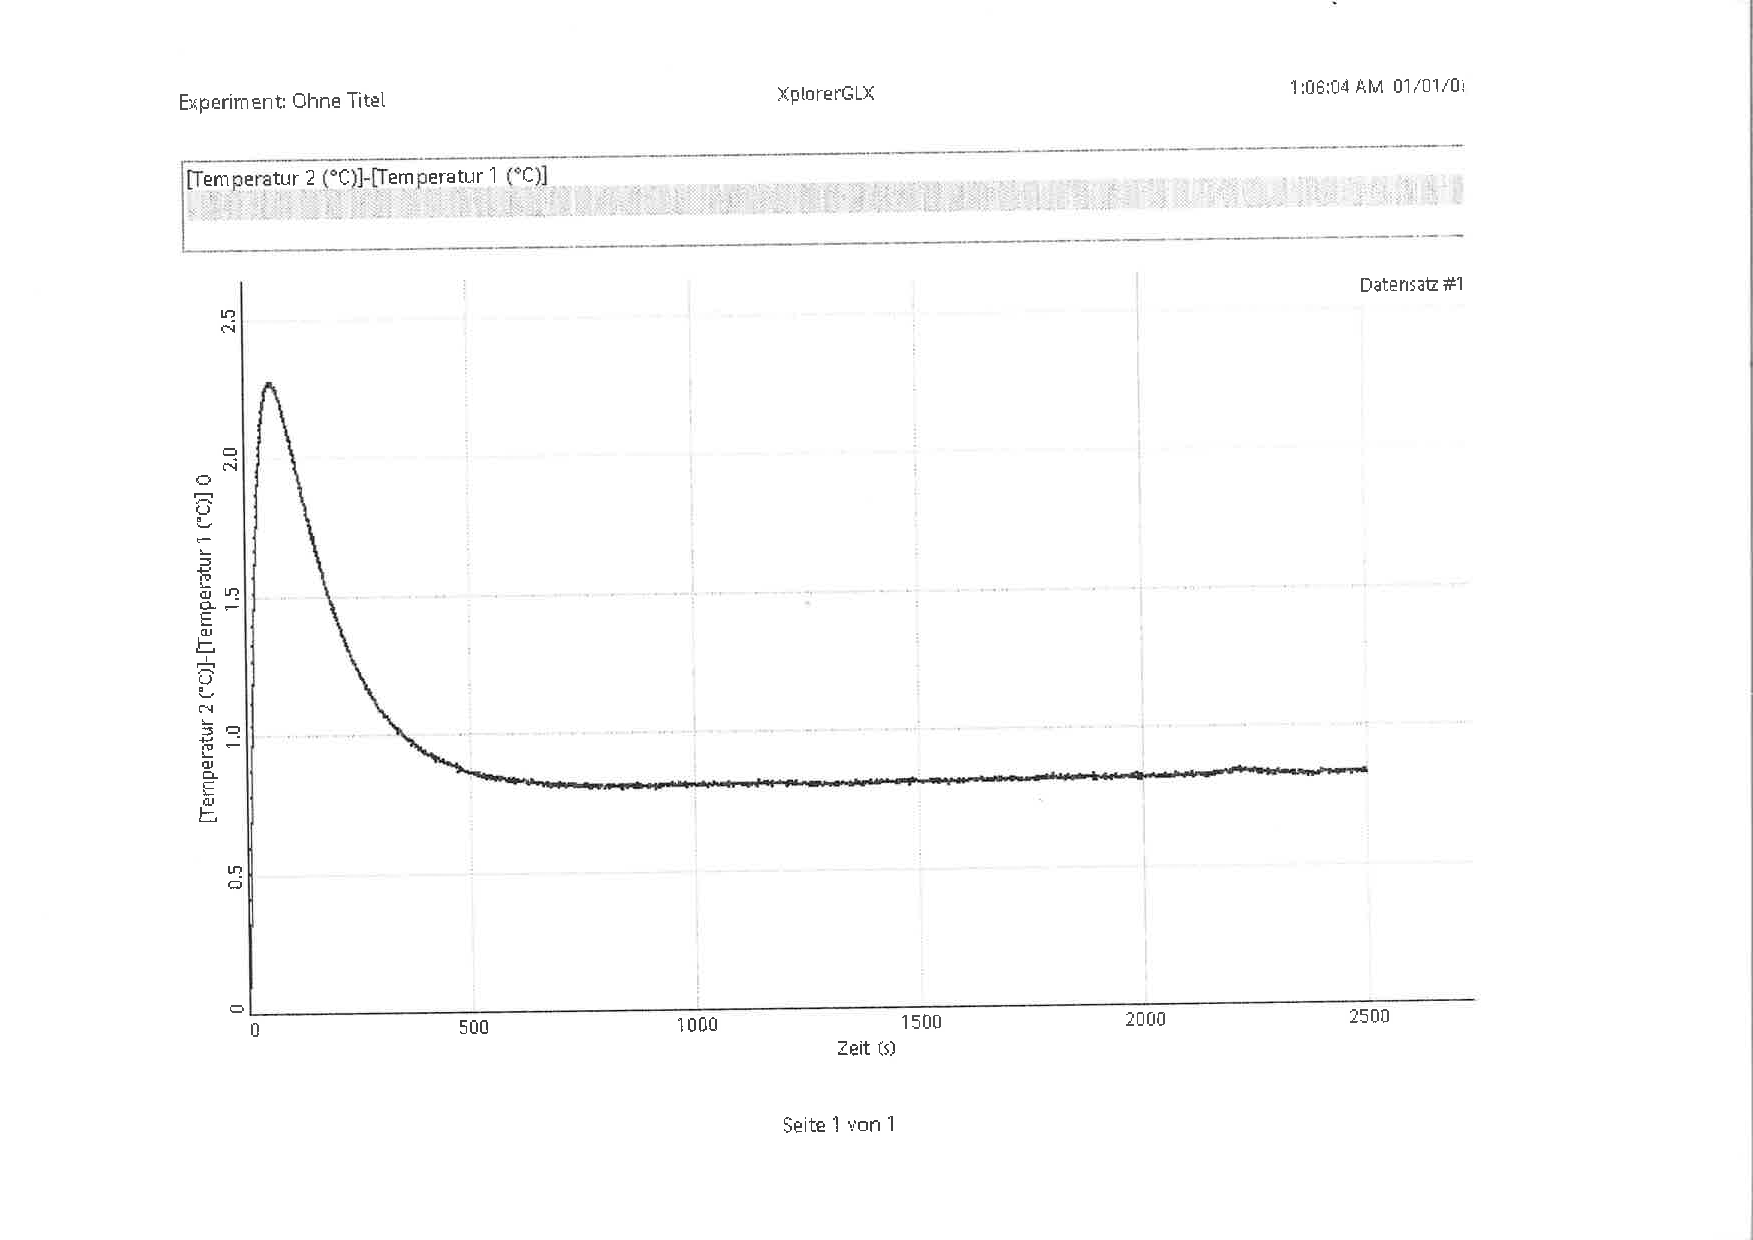
\includegraphics[width=\linewidth-70pt,height=\textheight-70pt,keepaspectratio]{content/Bilder/T2-T1-rotated.pdf}
	\label{fig:Graph3}
\end{figure}
\begin{table}
	\centering
	\caption{Der nach Formel \eqref{eq:form1} berechnete Wärmestrom $\frac{\Delta Q_{21}}{\Delta t}$ nach der Zeit $t$ und die aus \ref{fig:Graph3} entnommene Temperaturdifferenz $T2-T1$ bei dem breitem Messingstab.}
	\input{./build/tabT21.tex}
\end{table}
\begin{figure}
	\centering
	\caption{Die Temperaturdifferenz $T7-T8$ bei dem Edelstahlstab gegen die vergangene Zeit $t$ aufgetragen.}
	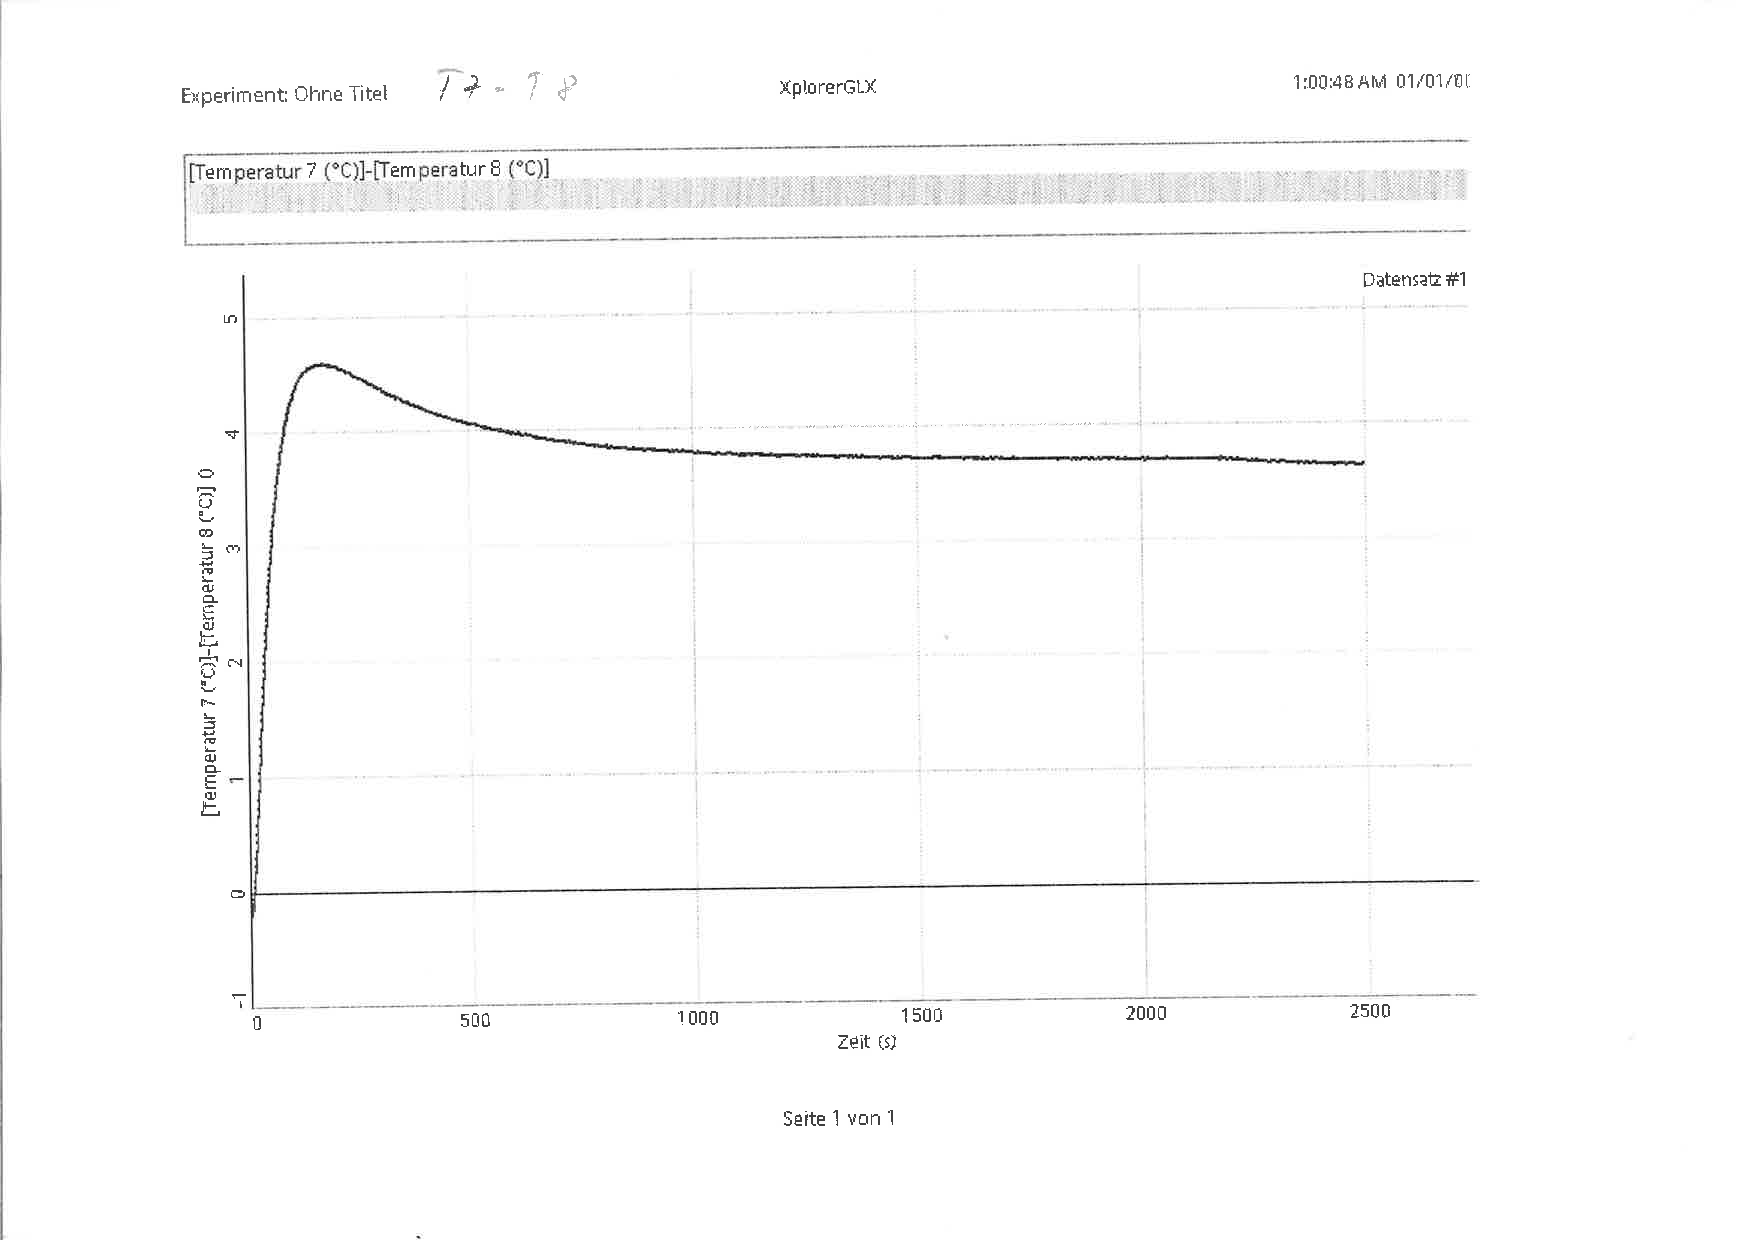
\includegraphics[width=\linewidth-70pt,height=\textheight-70pt,keepaspectratio]{content/Bilder/T7-T8-rotated.pdf}
	\label{fig:Graph4}
\end{figure}
\begin{table}
	\centering
	\caption{Der nach Formel \eqref{eq:form1} berechnete Wärmestrom $\frac{\Delta Q_{78}}{\Delta t}$ nach der Zeit $t$ und die aus \ref{fig:Graph4} entnommene Temperaturdifferenz $T7-T8$ bei dem Edelstahlstab.}
	\input{./build/tabT78.tex}
\end{table}

Der Wärmestrom $\frac{\Delta Q}{\Delta t}$ wurde in den Tabellen \ref{tab:tabT21} und \ref{tab:tabT78} mithilfe von Formel \eqref{eq:form1} berechnet. Hierfür wurde in beiden Tabellen die Temperaturdifferenz durch den vorher gemessenen Abstand zwischen den Thermoelementen $\Delta x$ von $\SI{3}{\centi\meter}$ geteilt. In Tabelle \ref{tab:tabT21} wurden die Querschnittsfläche $A$ von $\SI{0.48}{\centi\meter\squared}$, die Dichte $p$ von $\SI{8520}{\kilo\gram\per\meter\tothe{3}}$ und die spezifische Wärme $c$ von $\SI{385}{\joule\per\kilo\gram\per\kelvin}$ von Messing aus der Versuchsanleitung \cite{V204} und der Literaturwert für die Wärmeleitfähigkeit $\kappa$ von $\SI{93}{\watt\per\meter\per\kelvin}$ \cite{??} für die Berechnung verwendet.
In Tabelle \ref{tab:tabT78} wurden die Querschnittsfläche $A$ von $\SI{0.48}{\centi\meter\squared}$, die Dichte $p$ von $\SI{8000}{\kilo\gram\per\meter\tothe{3}}$ und die spezifische Wärme $c$ von $\SI{400}{\joule\per\kilo\gram\per\kelvin}$ von Edelstahl aus der Versuchsanleitung \cite{V204} und der Literaturwert für die Wärmeleitfähigkeit $\kappa$ von $\SI{20}{\watt\per\meter\per\kelvin}$ \cite{??} für die Berechnung verwendet. 
\subsection{Dynamische Methode}
\begin{figure}
	\centering
	\caption{Die Temperatur, am nahem Thermoelement des Messingstabes, $T2$ und, am fernem Thermoelement, $T1$ gegen die vergangene Zeit $t$ aufgetragen.}
	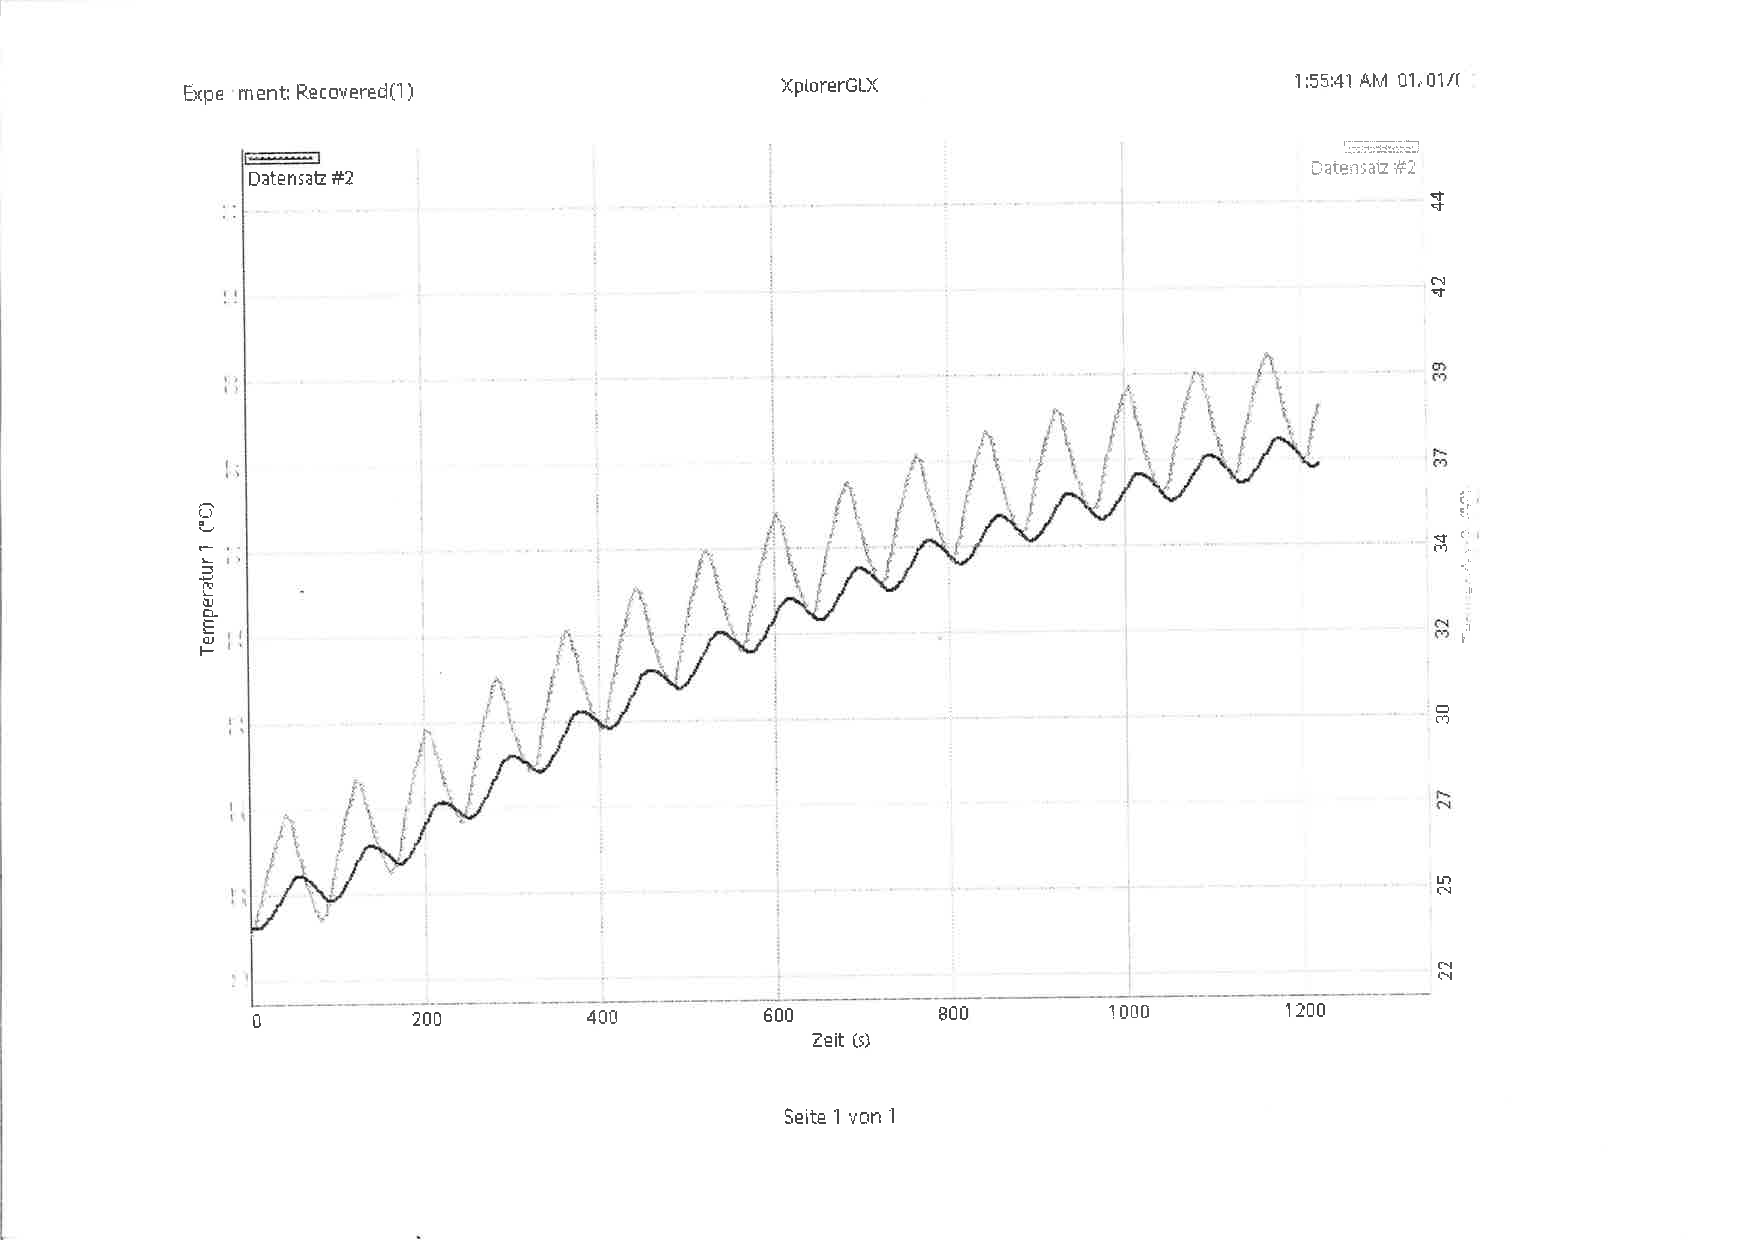
\includegraphics[width=\linewidth-70pt,height=\textheight-70pt,keepaspectratio]{content/Bilder/T1T2-rotated.pdf}
	\label{fig:Graph5}
\end{figure}
\begin{table}
	\centering
	\caption{Die aus dem Graphen in Abbildung \ref{fig:Graph5} entnommenen Werte für die Phasendifferenz $\Delta t$ die Amplitude am nahem Thermoelement des breitem Messingstabes $A_\text{nah}$ und am fernem Thermoelement $A_\text{fern}$.}
	\input{./build/tabMessing.tex}
\end{table}

Aus Tabelle \ref{tab:tabMessing} ergibt sich für die Amplitude am nahem Thermoelement des breitem Messingstabes:
\begin{displaymath}
A_\text{nah} = \SI{1.72(1)}{\kelvin}\text{,}
\end{displaymath}
für die Amplitude am fernem Thermoelement:
\begin{displaymath}
A_\text{fern} = \SI{0.557(6)}{\kelvin}
\end{displaymath}
und für die Phasendifferenz:
\begin{displaymath}
\Delta t = \SI{10.5(4)}{\second}\text{.}
\end{displaymath}
Damit berechnet sich die Wärmeleitfähigkeit von Messing mit den Werten aus der Versuchsanleitung \cite{V204} für die Dichte $p$ von $\SI{8520}{\kilo\gram\per\meter\tothe{3}}$ und der spezifischen Wärme $c$ von $\SI{385}{\joule\per\kilo\gram\per\kelvin}$ zu:
\begin{displaymath}
\kappa_\text{Messing} = \SI{125(5)}{\watt\per\meter\per\kelvin}\text{.}
\end{displaymath}
\begin{figure}
	\centering
	\caption{Die Temperatur, am nahem Thermoelement des Aluminiumstabes, $T6$ und, am fernem Thermoelement, $T5$ gegen die vergangene Zeit $t$ aufgetragen.}
	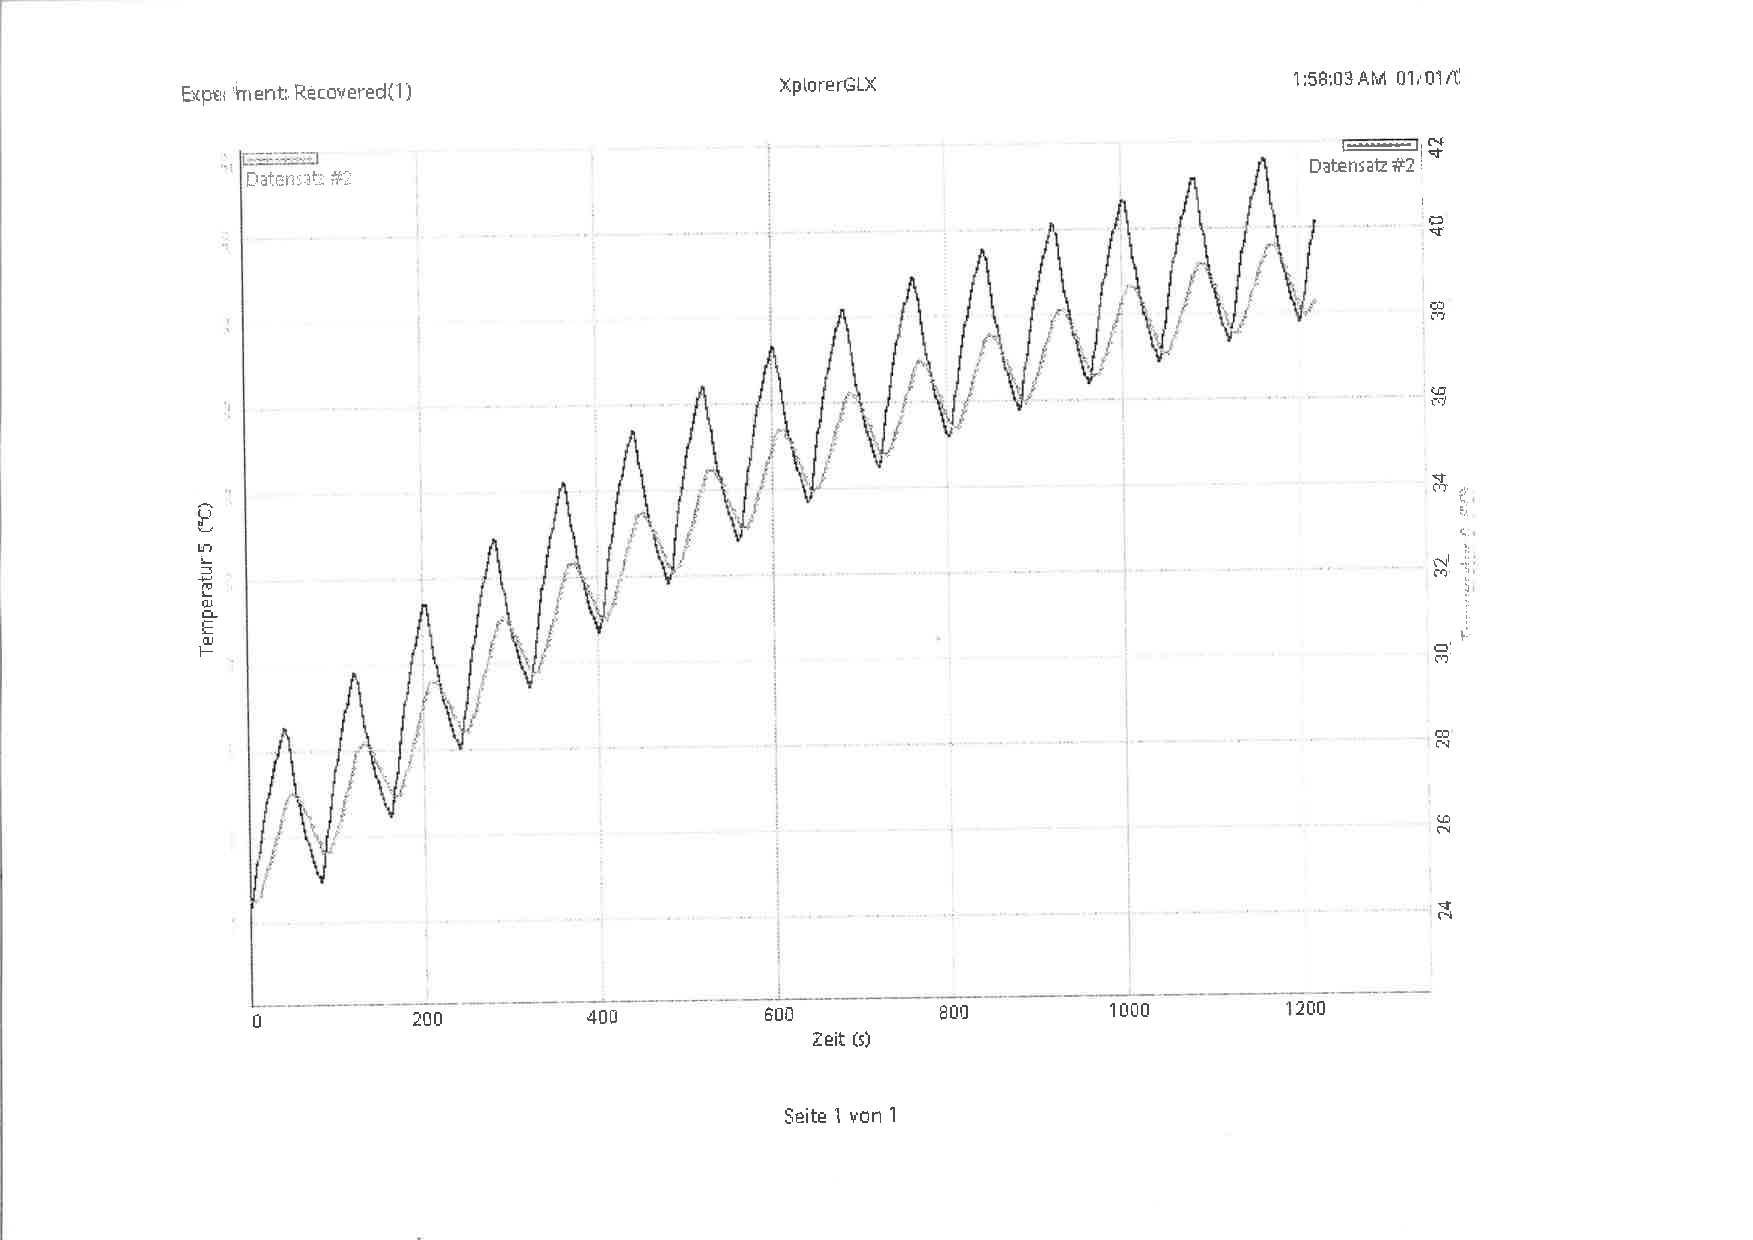
\includegraphics[width=\linewidth-70pt,height=\textheight-70pt,keepaspectratio]{content/Bilder/T5T6-rotated.pdf}
	\label{fig:Graph6}
\end{figure}
\begin{table}
	\centering
	\caption{Die aus dem Graphen in Abbildung \ref{fig:Graph6} entnommenen Werte für die Phasendifferenz $\Delta t$ die Amplitude am nahem Thermoelement des Aluminiumstabes $A_\text{nah}$ und am fernem Thermoelement $A_\text{fern}$.}
	\input{./build/tabAluminium.tex}
\end{table}

Aus Tabelle \ref{tab:tabAluminium} ergibt sich für die Amplitude am nahem Thermoelement des Aluminiumstabes:
\begin{displaymath}
A_\text{nah} = \SI{2.580(4)}{\kelvin}\text{,}
\end{displaymath}
für die Amplitude am fernem Thermoelement:
\begin{displaymath}
A_\text{fern} = \SI{1.19(1)}{\kelvin}
\end{displaymath}
und für die Phasendifferenz:
\begin{displaymath}
\Delta t = \SI{6.7(0)}{\second}\text{.}
\end{displaymath}
Damit berechnet sich die Wärmeleitfähigkeit von Aluminium mit den Werten aus der Versuchsanleitung \cite{V204} für die Dichte $p$ von $\SI{2800}{\kilo\gram\per\meter\tothe{3}}$ und der spezifischen Wärme $c$ von $\SI{830}{\joule\per\kilo\gram\per\kelvin}$ zu:
\begin{displaymath}
\kappa_\text{Aluminium} = \SI{202(3)}{\watt\per\meter\per\kelvin}\text{.}
\end{displaymath}
\begin{figure}
	\centering
	\caption{Die Temperatur, am nahem Thermoelement des Edelstahlstabes, $T7$ und, am fernem Thermoelement, $T8$ gegen die vergangene Zeit $t$ aufgetragen.}
	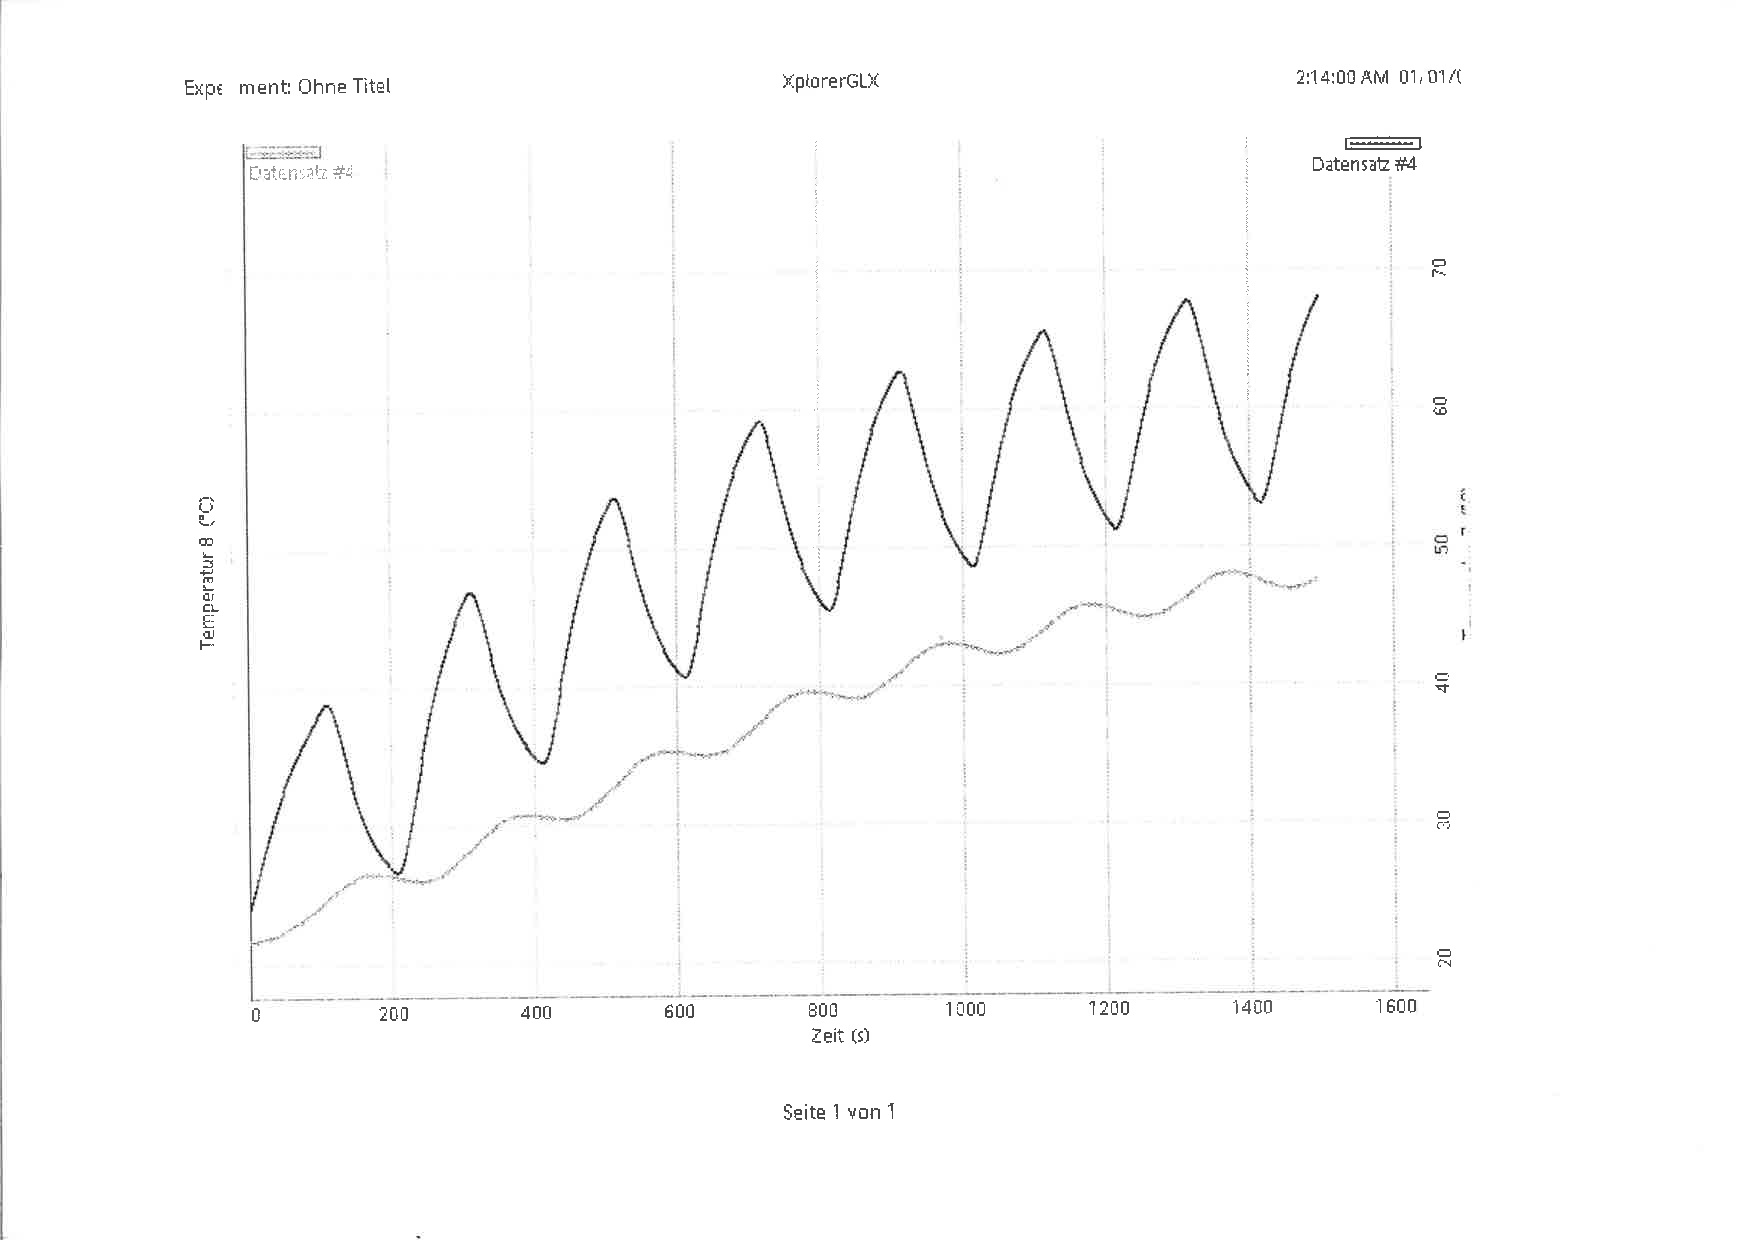
\includegraphics[width=\linewidth-70pt,height=\textheight-70pt,keepaspectratio]{content/Bilder/T7T8-rotated.pdf}
	\label{fig:Graph7}
\end{figure}
\begin{table}
	\centering
	\caption{Die aus dem Graphen in Abbildung \ref{fig:Graph7} entnommenen Werte für die Phasendifferenz $\Delta t$ die Amplitude am nahem Thermoelement des Edelstahlstabes $A_\text{nah}$ und am fernem Thermoelement $A_\text{fern}$.}
	\input{./build/tabEdelstahl.tex}
\end{table}

Aus Tabelle \ref{tab:tabEdelstahl} ergibt sich für die Amplitude am nahem Thermoelement des Edelstahlstabes:
\begin{displaymath}
A_\text{nah} = \SI{8.12(5)}{\kelvin}\text{,}
\end{displaymath}
für die Amplitude am fernem Thermoelement:
\begin{displaymath}
A_\text{fern} = \SI{1.1(0)}{\kelvin}
\end{displaymath}
und für die Phasendifferenz:
\begin{displaymath}
\Delta t = \SI{55(2)}{\second}\text{.}
\end{displaymath}
Damit berechnet sich die Wärmeleitfähigkeit von Edelstahl mit den Werten aus der Versuchsanleitung \cite{V204} für die Dichte $p$ von $\SI{8000}{\kilo\gram\per\meter\tothe{3}}$ und der spezifischen Wärme $c$ von $\SI{400}{\joule\per\kilo\gram\per\kelvin}$ zu:
\begin{displaymath}
\kappa_\text{Edelstahl} = \SI{12.9(5)}{\watt\per\meter\per\kelvin}\text{.}
\end{displaymath}